\begin{frame}[t]\label{a.2}
\frametitle{A Dynamics-Based Perspective: Dynamical Facilitation Theory}

DF theory (Chandler and Garrahan, \textit{Annu. Rev. Phys. Chem}, 2010) can explain glassy dynamics \textbf{without knowledge of local structure} with two key ideas:


% \only<5->
% {
% \begin{block}{\centering Highlights of DF Theory}
% \uncover<6->{Requires no knowledge of local structure or static properties.} \uncover<7->{Guided by kinetically-constrained lattice models, e.g., the Arrow model (Garrahan and Chandler, \textit{PNAS}, (2003)), to make predictions.}
% %, that captures the idea of facilitating excitations. }
% \end{block}
% }%\vspace{9pt}

\begin{columns}[T]
\begin{column}[T]{0.5\textwidth}

\onslide<2->\centering\textbf{\Large Excitations}

\begin{figure}[t]
\begin{overprint}

\onslide<2>\centering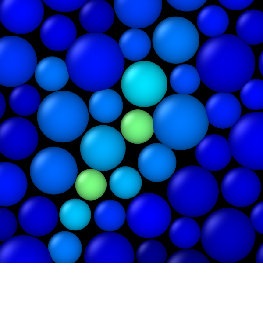
\includegraphics[height=0.525\textheight]{a.2-intro_dftheory/DF_Theory_Excitations_Zoom_0.pdf}\caption{Below the onset temperature $T_\mathrm{o}$, localized excitations drive glassy dynamics! (Keys, et al. \textit{Phys. Rev. X} 2011)}

\onslide<3>\centering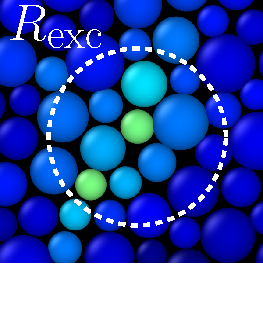
\includegraphics[height=0.525\textheight]{a.2-intro_dftheory/DF_Theory_Excitations_Zoom_1.pdf}\caption{Below the onset temperature $T_\mathrm{o}$, localized excitations drive glassy dynamics! (Keys, et al. \textit{Phys. Rev. X} 2011)}

\onslide<4->\centering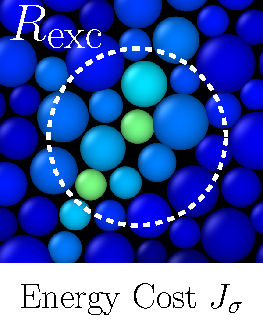
\includegraphics[height=0.525\textheight]{a.2-intro_dftheory/DF_Theory_Excitations_Zoom_2.pdf}\caption{Below the onset temperature $T_\mathrm{o}$, localized excitations drive glassy dynamics! (Keys, et al. \textit{Phys. Rev. X} 2011)}


\end{overprint}
\end{figure}

\end{column}
%\vrule{}
\begin{column}[T]{0.50\textwidth}

\onslide<5->\centering\textbf{\Large Facilitation}
\begin{figure}[t]
\begin{center}
\begin{overprint}
\onslide<5>\centerline{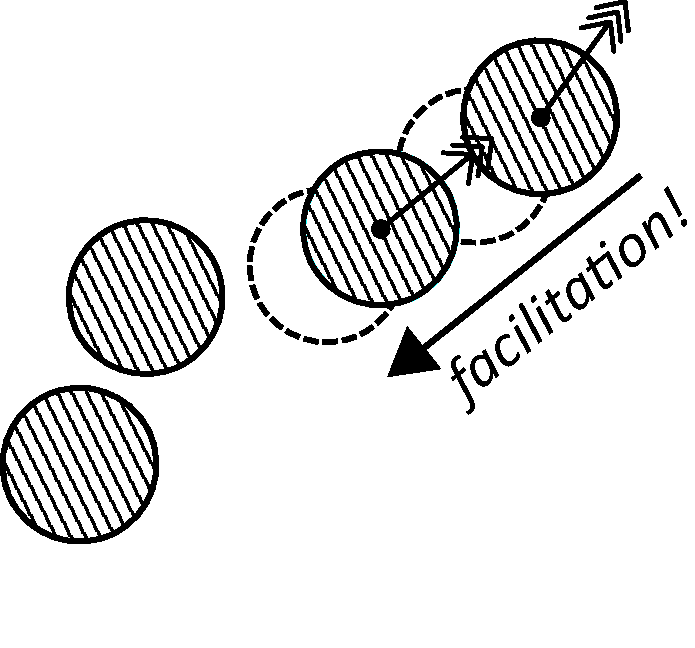
\includegraphics[height=0.525\textheight]{a.2-intro_dftheory/facilitation_closer_1.pdf}}
\onslide<6->\centerline{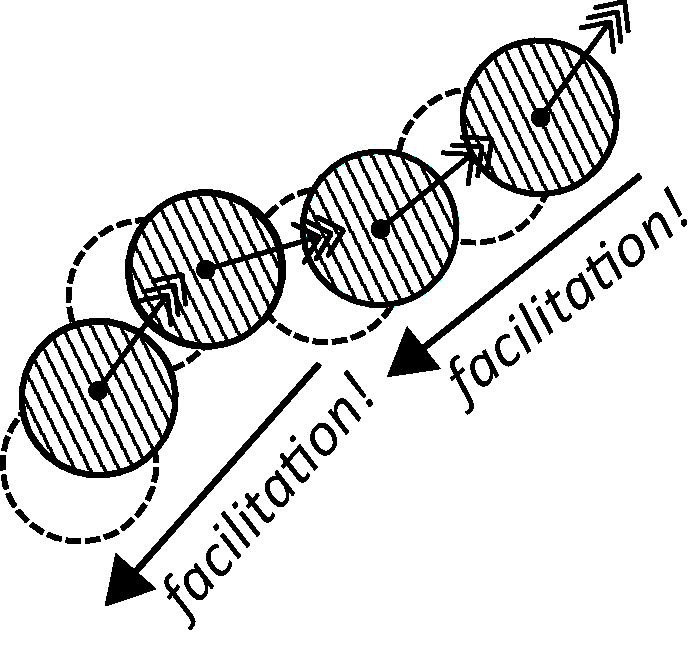
\includegraphics[height=0.525\textheight]{a.2-intro_dftheory/facilitation_closer_2.pdf}}
\end{overprint}
\end{center}
\caption{Excitations facilitate the creation and relaxation of another excitation close by.}
\end{figure}

\end{column}
\end{columns}

\end{frame}